
\begin{figure}[t]
    \centering
        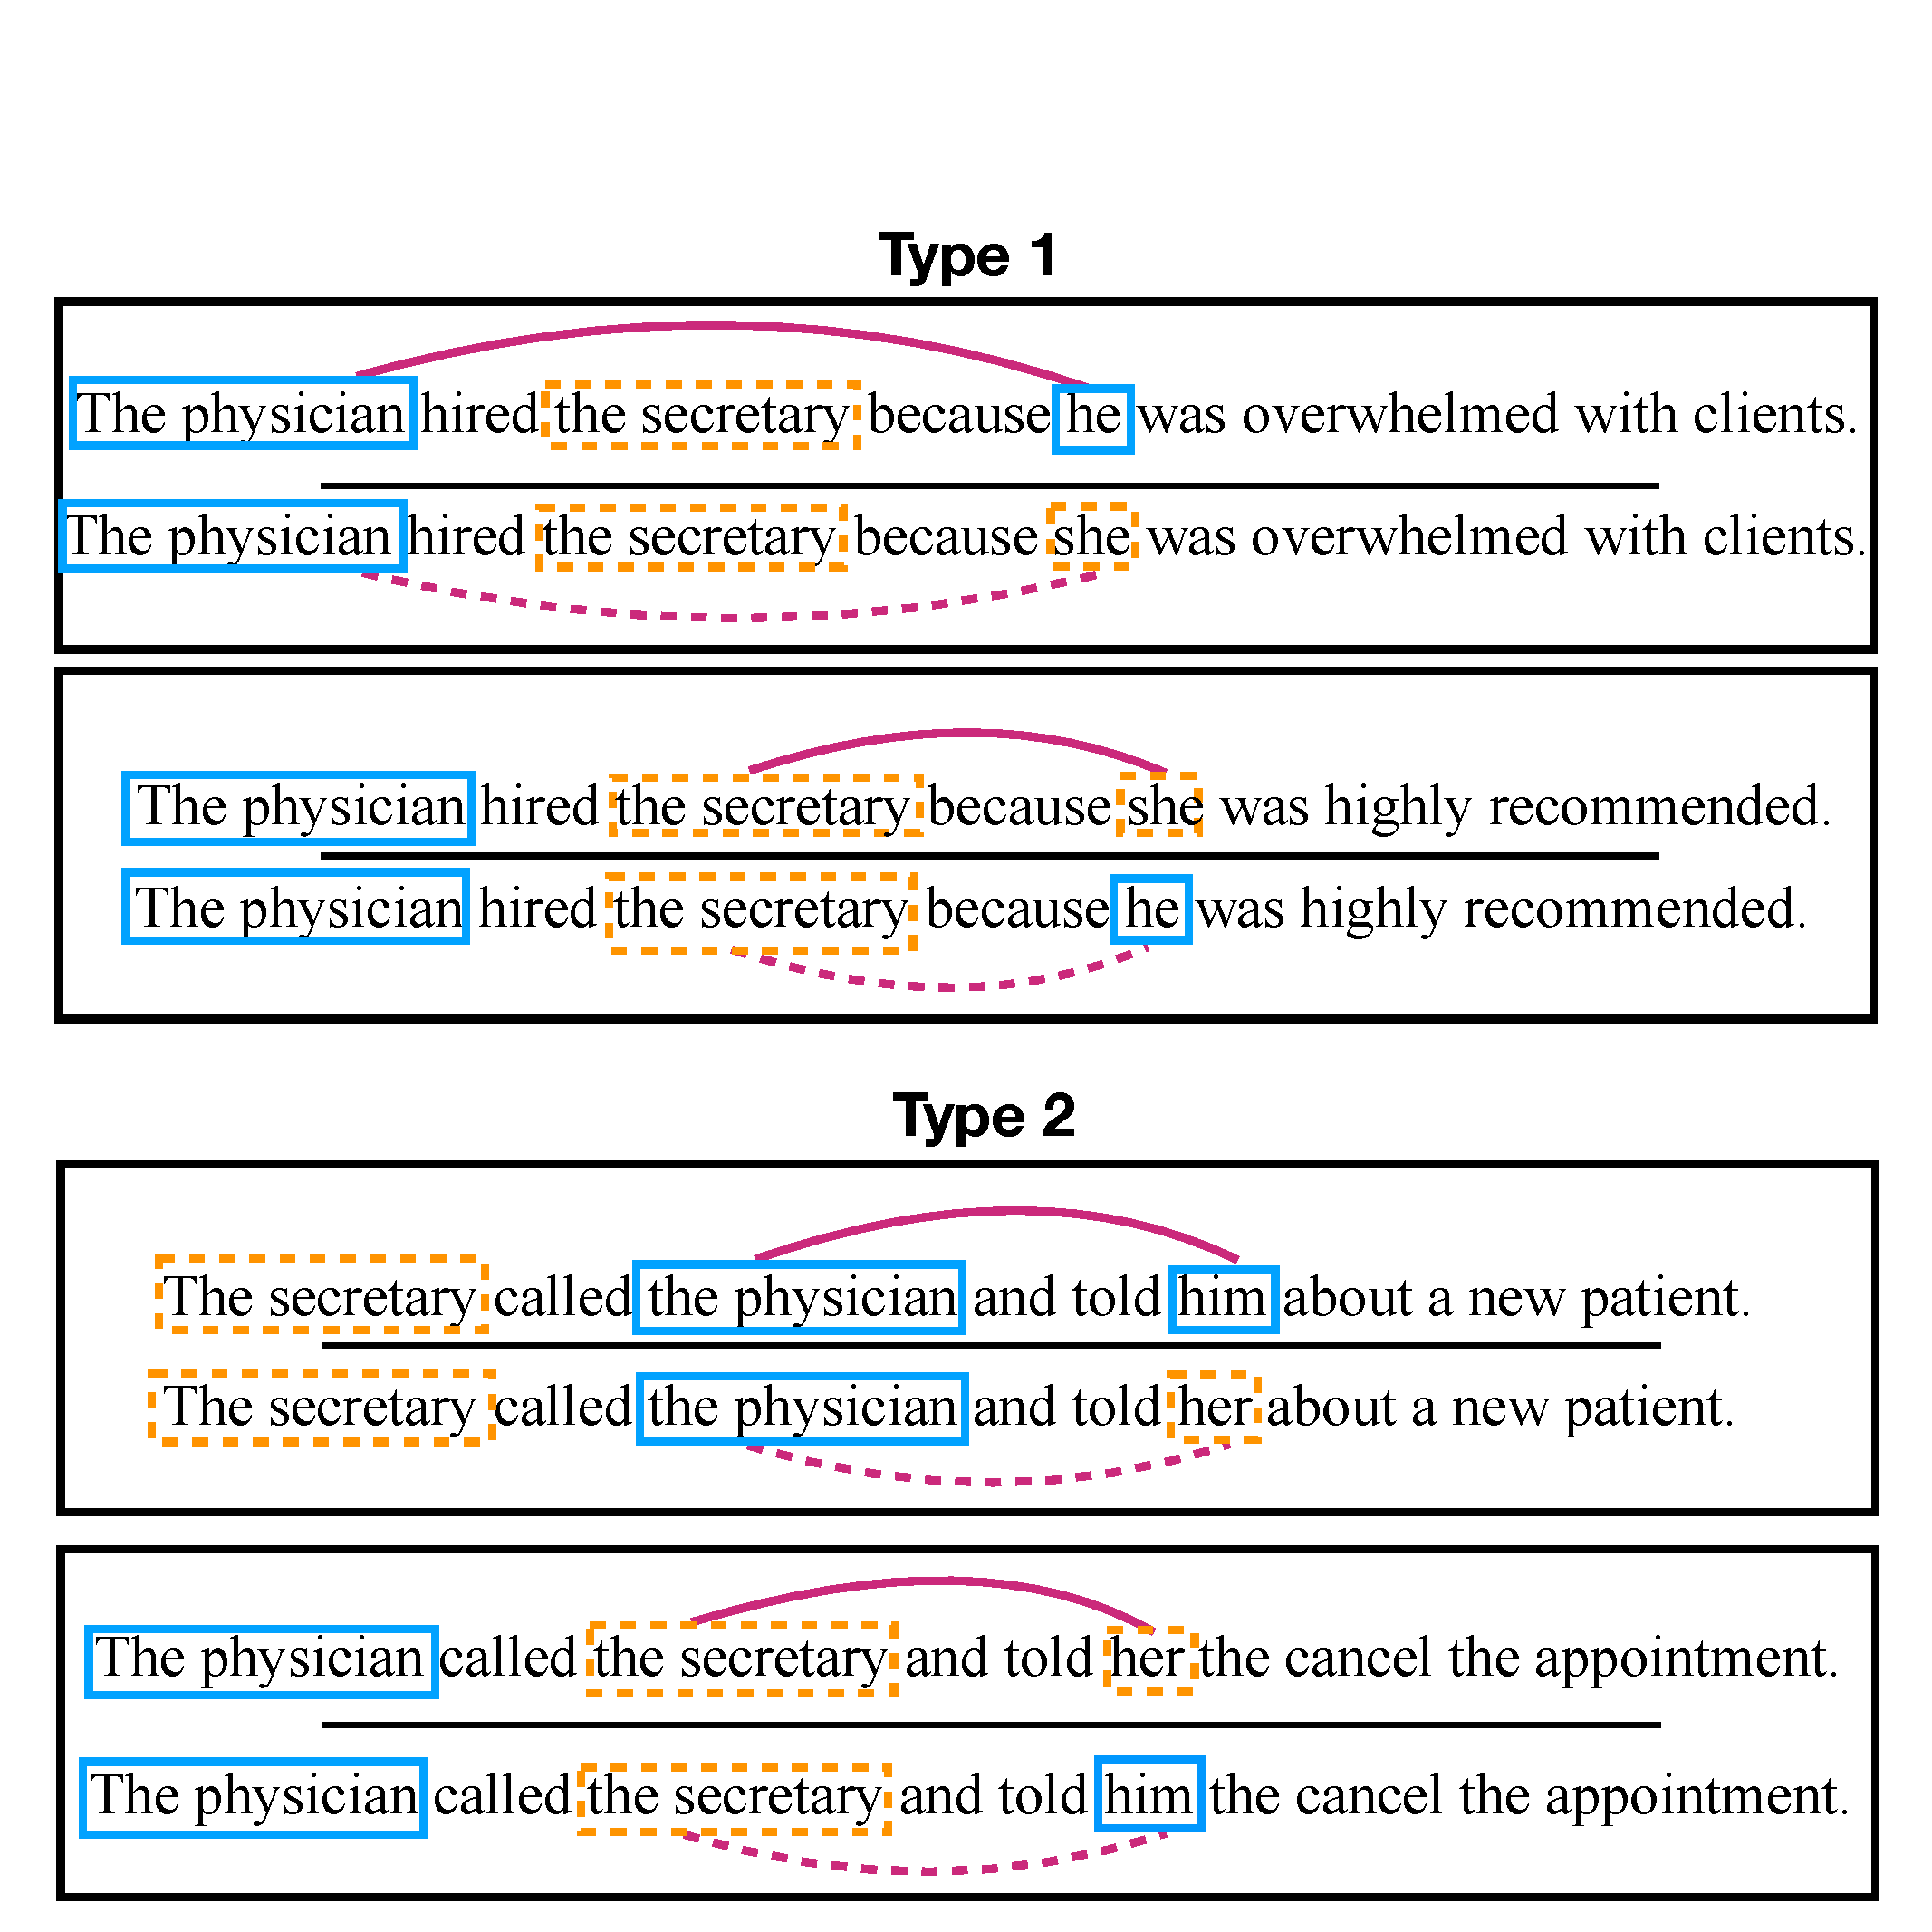
\includegraphics[width=\linewidth]{figures/coref_bias_teaser2.pdf}
        \vspace{-20pt}
        \label{fig:president_he}
    \caption{\small Pairs of gender balanced co-reference tests in the~\dataset~dataset. Male and female entities are marked in solid blue and dashed orange, respectively. For each example, the gender of the pronominal reference is irrelevant for the co-reference decision. Systems must be able to make correct linking predictions in pro-stereotypical scenarios (solid purple lines) and anti-stereotypical scenarios (dashed purple lines) equally well to pass the test. Importantly, stereotypical occupations are considered based on US Department of Labor statistics.}
    \vspace{-10pt}
\label{fig:teaser}
\end{figure}

%However, despite these models demonstrating strong results, we observe that they make systematic errors on gender pronouns, revealing that the systems exhibit sexual bias. 

%This task aims at finding noun phrases or mentions referring to the same entity in a document. 
% For instance, let us consider the following paragraph~\cite{Chang15}:
% \textit{
% (ENGLAND, June, 1989) - [\underline{Christopher Robin}] is alive and well. \underline{He} lives in
% England. \underline{He} is the same person that you read about in the book, Winnie the Pooh. As
% a boy, \underline{Chris} lived in a pretty home called Cotchfield Farm. When [\underline{Chris}] was three
% years old, \underline{his} father wrote a poem about \underline{him}. The poem was printed in a magazine for
% others to read. [Mr. Robin] then wrote a book. He made up a fairy tale land where
% \underline{Chris} lived. \underline{His} friends were animals. There was a bear called Winnie the Pooh. There
% was also an owl and a young pig, called a piglet. All the animals were stuffed toys that \underline{Chris} owned.}
% All the underlined mentions in the given paragraph refer to the same entity -- Christopher Robin. Therefore, a coreference resolution system will group them in the same cluster. Coreference resolution, in essence, aims at generating a clustering, such that mentions for the same entity are in the same class. 
%It has been a long-lasting problem~\cite{ng2010supervised} in natural language processing and various approaches, including rule-based~\cite{raghunathan2010multi}, feature-based~\cite{DurrettKlein2013,PengChRo15}, and neural-network based methods~\cite{clark2016deep,lee2017end}, have been proposed. 
%Existing approaches often aim at improving the overall performance of generating coreference clusters over the entire corpus. However, despite these models demonstrating strong results, we observe that they make systematic errors on gender pronouns, and lead to gender-biased predictions. 
% Specifically, given the same context, the system behaves differently with respect to different gender pronouns. 
%For instance, the two paragraphs in Figure~\ref{fig:president} are almost identical.
%In the first sentence, the system successfully identifies that the male pronoun ``his'' refers to ``President''. However, in the second paragraph, the same system fails to associate the female pronoun ``her'' with ``President''. 
%Similarly, the system makes stereotypical predictions with respect to pronominal references when dealing with other job titles, such as leader, minister, and teacher. 


%% maybe move the following paragraph to conclusion??
%Biased predictions from a coreference resolution system risk being propagated to downstream applications, such as information extraction, machine reading comprehension, and machine translation.
%For example, a relation extraction system that successfully identifies a ``work-for'' relationship between a male agent and a tech company may fail to do the same thing for a female agent even when the context is the same.
%If statistics collected by such a biased system are used in downstream tasks, something unexpected may happen. For instance, automatic resume filtering systems may inadvertently be affected by the gender and ethnicity of the pool of applicants.

% \begin{figure*}[t]
%     \centering
%         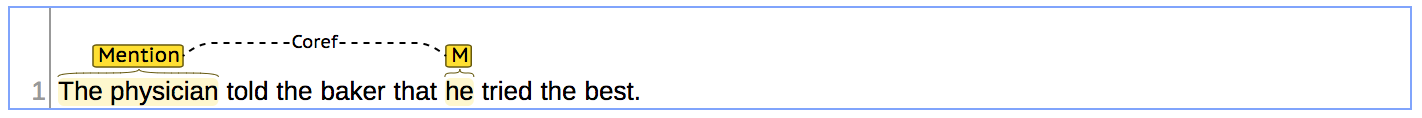
\includegraphics[width=\linewidth]{figures/physician_he.png}
%         \label{fig:president_he}
%         
\includegraphics[width=\linewidth]{figures/physician_she.png}
%         \label{fig:president_she}
%     \caption{When providing the Stanford coreference system with exact same information but the gender, the predictions are different. The system can correctly build the connection between ``physician'' and ``he'' but not for ``she''.}
% \label{fig:president}
% \end{figure*}


%For UW e2e system:
%Document text: President, outside the Calvary Chapel church, praised the recovery effort after Hurricane Maria. She  compared Puerto Rico to other storms that have killed far more people, even though, she said, they weren't perhaps as strong. At her side were Puerto Rico's governor and local officials.
%Predicted cluster: ['Hurricane Maria', 'She', 'she', 'her']
%Predicted cluster: ['Puerto Rico', "Puerto Rico 's"]
% Document text: President, outside the Calvary Chapel church, praised the recovery effort after Hurricane Maria.He  compared Puerto Rico to other storms that have killed far more people, even though, he said, they weren't perhaps as strong. At his side were Puerto Rico's governor and local officials.
% Predicted cluster: ['President , outside the Calvary Chapel church ,', 'he', 'his']
% Predicted cluster: ['Puerto Rico', "Puerto Rico 's"]
 
 

%% KW: mention the new dataset, cite the following two winograd papers: \cite{RahmanNg12c,peng2015solving}


% Machine learning models are often built so that
% they generalize observations from the data they are
% trained on. 
% Generalization allows models to make
% predictions on unseen instances at test time.
% However,
% when such generalization ability is applied
% to variables such as gender, age, or race, there is
% a risk of making biased decisions based on general
% impressions of a demographic group.
% Several instances of this problem have been demonstrated
% in previous works


Coreference resolution is a task aimed at identifying phrases (mentions) referring to the same entity. %, has been a fundamental task in NLP. % and has been adopted in a wide range of applications, including  document summarization, question answering and information extraction~\cite{bengtson2008understanding,lee2011stanford}.
Various approaches, including rule-based~\cite{raghunathan2010multi}, feature-based~\cite{DurrettKlein2013,PengChRo15}, and neural-network based ~\cite{clark2016deep,lee2017end} have been proposed. 
While significant advances have been made, systems carry the risk of relying on societal stereotypes present in training data that could significantly impact their performance for some demographic groups.

In this work, we test the hypothesis that co-reference systems exhibit gender bias by creating a new challenge corpus, \dataset.%\footnote{{https://uclanlp.github.io/corefBias/}}
This dataset follows the winograd format~\cite{hirst,RahmanNg12c,peng2015solving}, and contains references to people using a vocabulary of 40 occupations.
It contains two types of challenge sentences that require linking gendered pronouns to either male or female stereotypical occupations (see the illustrative examples in Figure~\ref{fig:teaser}).
None of the examples can be disambiguated by the gender of the pronoun but this cue can potentially distract the model. 
%and each type contains both stereotype and non\_stereotype subset.
We consider a system to be gender biased if it links pronouns to occupations dominated by the gender of the pronoun (pro-stereotyped condition) more accurately than occupations not dominated by the gender of the pronoun (anti-stereotyped condition).
%\my{I want to add a sentence here about that we are providing a weak certification, but it sounds very negative here Maybe : Our corpus can be used to certify a system has gender bias but we are unable to certify systems are gender bias free. (my : I like that lot) How about: }
The corpus can be used to certify a system has gender bias.\footnote{Note that the counter argument (i.e., systems are gender bias free) may not hold.}
%Such a test provides a weak guarantee 
%The dataset is large, containing over 3000 sentences.

We use three different systems as prototypical examples: the Stanford Deterministic Coreference System~\cite{raghunathan2010multi}, the Berkeley Coreference Resolution System~\cite{DurrettKlein2013} and the current best published system: the UW End-to-end Neural Coreference Resolution System~\cite{lee2017end}.
Despite qualitatively different approaches, all systems exhibit gender bias, showing an average difference in performance between pro-stereotypical and anti-stereotyped conditions of $21.1$ in F1 score.
Finally we show that given sufficiently strong alternative cues, systems can ignore their bias. 
%\jy{Concurrent work~\cite{Rachel18} also shows bias in coreference resolution systems.}

%it should provide similar results on these two subsets. However, the aforementioned models all show great difference on the stereotype and non\_stereotype datasets which also prove the potential gender bias issue.
In order to study the source of this bias, we analyze the training corpus used by these systems, Ontonotes 5.0~\cite{weischedel2012ontonotes}.\footnote{The corpus is used in CoNLL-2011 and CoNLL-2012 shared tasks, http://www.conll.org/previous-tasks} Our analysis shows that female entities are significantly underrepresented in this corpus. % and it exhibits strong gender biases.
To reduce the impact of such dataset bias, we propose to generate an auxiliary dataset where all male entities are replaced by female entities, and vice versa, using a rule-based approach.
Methods can then be trained on the union of the original and auxiliary dataset.
In combination with methods that remove bias from fixed resources such as word embeddings~\cite{BCWS16}, our data augmentation approach completely eliminates bias when evaluating on \dataset~, without significantly affecting overall coreference accuracy. 

%\my{I think we want to emphasize our code and data are avaiable here: How about we move the footnote 1 to here and say somethign like: The code and data are available at \url{http://winobias.org.}}
%We further demonstrate that models trained on this corpus inherit the bias and make systematic errors when resolving coreference. 



%Besides showing there is stereotype in the above coreference resolution systems, we also build a new benchmark dataset, which can be used to reveal the gender biases in different systems. 


%Inspired by the example in Figure~\ref{fig:president}, we generate a gender-reversed corpus where the male pronouns and female pronouns are exchanged. 
%We find that all three coreference resolution systems perform significantly worse on the reversed corpus than on the original one. This supports our hypothesis that coreference resolution systems are sensitive to the gender of entities in the text. 


%% KW: mention the debias scheme. 
%To reduce the impact of gender bias in coreference resolution systems, we propose different algorithms to neutralize the effect of gender imbalance in training data. 
%Specifically, ART retrains the model by using augmented training dataset. DRT algorithm applies the debiased word embeddings to the system and DART algorithm combines the above two algorithms.
% first generates a gender-reversed corpus by swapping male words with female words in the data and then training the coreference system on the union set of the original corpus and the gender-reversed corpus.
%Experimental results demonstrate that our proposed methods can help to reduce the biases and the DART algorithm achieves best performance in mitigating the bias.
% this new trained model can reduce biased predictions while maintaining the accuracy of the original model.


%While gender bias has been investigated in other tasks, to our best knowledge, this is the first work to tackle the gender bias issue in coreference resolution.
%Our contributions are summarized as follows:


% \begin{itemize}
% \item We analyze the corpus used for training coreference resolution systems. We show that the corpus exhibits strong gender bias. 
% \item We propose an evaluation procedure to test the gender bias of a coreference resolution system by exchanging male and female word pairs. 
% \item We propose an algorithm to calibrate the gender bias in coreference resolution systems. The approach reduces the bias in the system while maintaining its performance. 
% \end{itemize}